\documentclass[10pt]{article}

\usepackage{amsmath}
\usepackage{amssymb}
\usepackage{graphicx}
\usepackage{color} 
\usepackage{units}
\usepackage{setspace} 
\onehalfspacing

% Text layout
\topmargin -1.5cm
\oddsidemargin 0.5cm
\evensidemargin 0.5cm
\textwidth 16cm 
\textheight 23cm
\setlength{\parindent}{0pt}

% Bold the 'Figure #' in the caption and separate it with a period
% Captions will be left justified
\usepackage[labelfont=bf,labelsep=period,justification=raggedright]{caption}

\usepackage{jneurosci}
\bibliographystyle{jneurosci}

\title{Lecture 6: Tuning curves and population analysis}
\author{Caterina Trainito, Oleg Vinogradov}
\date{May 24, 2016}

\begin{document}

\maketitle

\section*{Introduction}

Most neurons in V1, including simple cells and complex cells, are selective for stimulus orientation or direction of motion \cite{hubel1962receptive}. These neurons respond preferentially to stimuli with a specific orientation, while their firing probability drops off with distance from the preferred range. At the population level, these neurons represent all possible orientations with overlapping tuning curves. This coding scheme maximizes information content \cite{snippe1996parameter} and thus allows for the highly sensitive edge detection \cite{marr1980theory}. \\

To explore the properties of orientation tuning, we analysed spike trains from monkey V1 cells in response to drifting gratings with varying direction of motion. After appropriate visualization of the data, we used several approaches to analyse individual neurons' orientation tuning and compare response properties across cells.
\paragraph{Linear model.} Since orientation is a circular variable, it can be represented as a vector on the unit circle defined by its trigonometric components. Firing rate can then be modelled as a linear function of the reparametrized stimulus orientation:
\begin{equation*}
f(x) = a+b^Tx
\end{equation*}
where 
\begin{align*}
b = \beta \begin{bmatrix}
cos (\phi) \\  sin (\phi )
 \end{bmatrix}  
 \hspace{5mm}
 x =  \begin{bmatrix}
cos (\theta) \\
  sin (\theta)
 \end{bmatrix} 
\end{align*}
which is equal to 
\begin{equation*}
f(\theta) = a+ \beta cos(\theta - \phi).
\end{equation*}
Where $\theta$ is the direction of motion and $\phi$ is the parameter of a model.\\

Alternatively, the same cosine tuning curve fit can be implemented by transferring the problem into the frequency domain. The tuning curve function is then given by the linear combination of the DC component and the second Fourier component:
\begin{equation*}
f = q_0+q_2v_2+ \bar{q_2}\bar{v_2}
\end{equation*}
whete $v$ is a complex exponential and $q$ denotes projection of the mean spike count.

This model, however, assumes Gaussian i.i.d. error terms. Taking into account the physiological properties of neuronal firing, the fit can be improved by modelling the noise as Poisson distributed \cite{softky1993highly}. This imposes the constraint that the estimated spike counts be non-negative, and, importantly, reflects the significant heteroscedasticity of the data.


\section*{Methods}

We analysed extracellularly recorded spike trains of 41 units from monkey V1. Activity was analysed in a 2000 msec window of stimulus presentation. Stimuli were Gabor patches of 2 deg diameter and 2-3 deg eccentricity, with a spatial frequency of 3 cyc/deg, drifting at a speed of 3.4 cyc/deg. The gratings could move in 16 directions of motion, equally spaced between 0 deg and 337.5 deg to cover the full range of orientations. Each condition consisted of 11 trials, for a total of 176 trials presented in randomized order. The resulting data consisted of a $11\times16$ spike count matrix and a $1\times16$ vector of motion directions in degrees.

\paragraph{Data visualization.} For a selection of neurons, we visualized the average spike count for each direction of motion in a linear plot. As a measure of dispersion, we included the individual counts of all 11 trials per condition.

\paragraph{Tuning curve fitting.} To roughly assess the periodicity of the neurons' orientation tuning, we fit a cosine tuning curve to the spike count data of each individual neuron. We took the Fourier transform of the data by projecting (up to the norm) the vector of mean counts onto a complex exponential with two cycles, representing the two expected peaks. This is equivalent to taking the inner product
\begin{equation*}
q = m^Tv
\end{equation*}
where $q$ is a projection of the mean spike count of each neuron $m = \frac{1}{n} \sum_j x_{jk}$ on a complex exponential $v = 1/4\exp \{2i \theta\} $. \\
The resulting tuning curve is given by
\begin{equation*}
f_k = \langle m \rangle + \bar{q} v_k + q \bar{v_k} 
\end{equation*}
with preferred oriention $\phi = \arg(q)$.

\paragraph{Linear-nonlinear model.} By adding an exponential nonlinearity, the L-NL model yields tuning curves that follows a von Mises distribution, or circular Gaussian. The full von Mises model, which includes a coefficient for the first harmonic, is given by
\begin{equation*}
f(\theta) = \exp\{ \alpha+\kappa(\cos(2(\theta-\phi))-1)+\nu(\cos(\theta-\phi)-1)\}
\end{equation*}
where $\theta$ is the direction and  $\alpha, \kappa, \nu, \phi$ are four parameters of the distribution. \\

We then implemented the von Mises model assuming Gaussian noise. The two-cycle von Mises distribution was fitted to spike count data from all trials by computing the least squares solution. \\
To fit the von Mises model within a Poisson noise model, we computed the maximum likelihood estimator
\begin{equation*}
\mathcal{L}(k,\lambda) = k\log(\lambda)-\lambda
\end{equation*}
As a cost function we calculated the negative log-likelihood of the Poisson distribution summed over all trials: 
\begin{equation*}
E = - \sum_n \mathcal{L}(k,\lambda)
\end{equation*}
where the mean parameter $\lambda$ is the estimated spike count given by the von Mises fit, $\lambda = f(\theta)$. We minimized the negative log-likelihood with respect to the four parameters of the von Mises function by computing the respective gradients:
\begin{align*}
 \frac{\partial L}{\partial \alpha} = &k - \lambda  \\
 \frac{\partial L}{\partial \kappa} = &k(\cos(2(\theta-\phi))-1) - ((\cos(2(\theta-\phi))-1) \lambda \\
 \frac{\partial L}{\partial \nu} = &k(\cos(\theta-\phi)-1) - ((\cos(\theta-\phi)-1)) \lambda \\
 \frac{\partial L}{\partial \phi} =  & k(2\kappa \sin(2(\theta-\phi)) - \nu \sin(\phi-\theta)) -(2\kappa \sin(2(\theta-\phi))- \nu \sin(\phi-\theta)) \lambda
\end{align*}

\paragraph{Test for orientation selectivity.} Within the linear Fourier model, we implemented a permutation test to assess statistically the cells' orientation selectivity. A total of 1000 iterations were performed. In each iteration, we randomly permuted all elements of the spike count matrix, equivalent to shuffling the trials' condition labels. From each shuffled dataset we computed the test statistic $|q|$, the modulus of the second Fourier component. The distribution of all calculated values of $|q|$ is an estimate of the null distribution for the test, i.e. the sampling distribution under the null hypothesis of random firing (no orientation tuning). For each cell, we then computed a p-value as the proportion of $|q|$ values that are equal to or more extreme than the observed value for that cell. Cells with p-values that cross the chosen significance threshold of 0.01 were classified as orientation-selective.

\section*{Results}
 
\paragraph{Tuning curve fitting.} The figures below show data and tuning curves from two example cells, cell 29 (significantly orientation-selective, $p<0.01$) and cell 1 (not significantly tuned, $p=0.70$). The plots include spike counts for all 176 trials and the average count for each stimulus condition.

\newpage

\begin{figure}[!h]
\centering
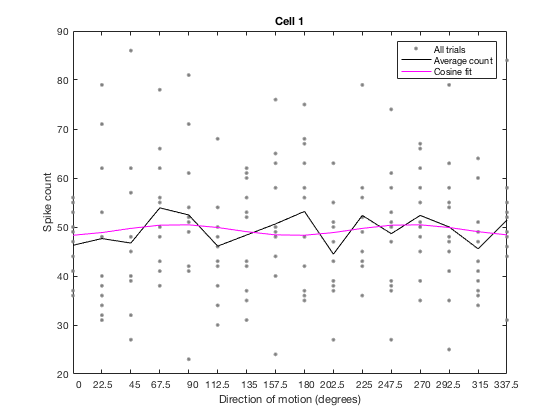
\includegraphics[height=10cm]{fitCosCell1.png}
\caption{Cosine tuning curve for cell 1 (not orientation selective).
\label{fitCos1}}
\end{figure}

\begin{figure}[!h]
\centering
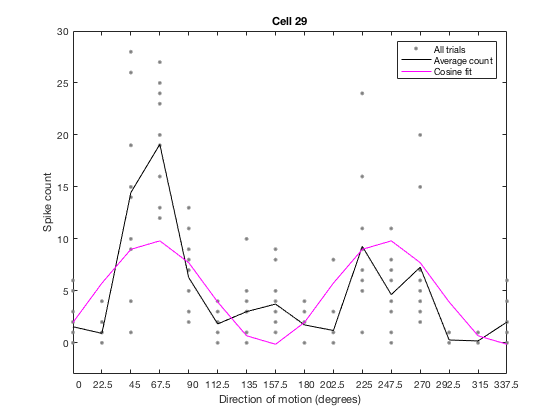
\includegraphics[height=10cm]{fitCos.png}
\caption{Cosine tuning curve for cell 29 (orientation selective).
\label{fitCos29}}
\end{figure}

\begin{figure}[!h]
\centering
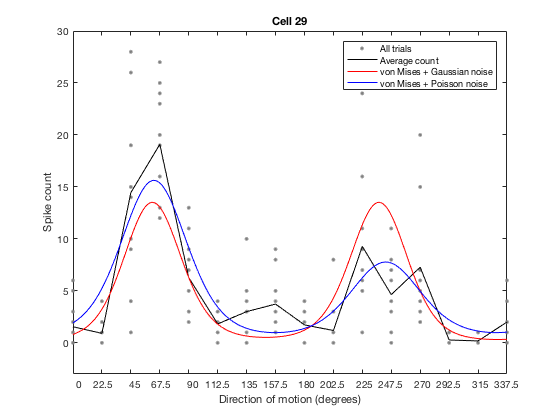
\includegraphics[height=10cm]{fitVonMises.png}
\caption{Von Mises tuning curves for cell 29.
\label{fitVonMises}}
\end{figure}

\paragraph{Test for orientation selectivity.} Running the permutation test on all cells of our dataset, 34 out of 41 cells were found to be tuned to orientation at an alpha level of 1\%. Figures~\ref{permplot29} and~\ref{permplot1} show the null distributions of $|q|$ computed for cell 29 (orientation-selective) and cell 1 (not orientation-selective).

\begin{figure}[!h]
\centering
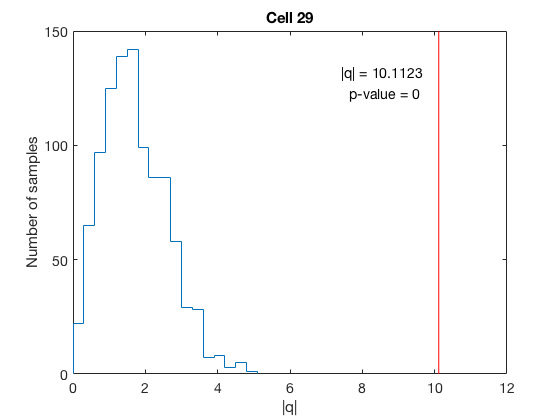
\includegraphics[height=7cm]{permplot.png}
\caption{Permutation test for cell 29. The histogram shows the of the test statistic $|q|$ generated by 1000 permutations of all trials' labels under the null hypothesis of random firing. The red line indicates the value of $|q|$ observed in the data for cell 29.
\label{permplot29}}
\end{figure}

\begin{figure}[!h]
\centering
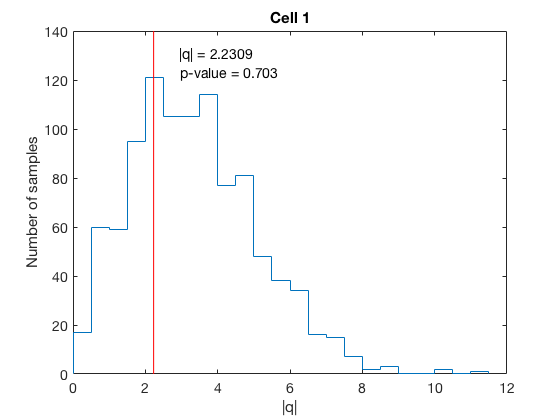
\includegraphics[height=7cm]{permplot1.png}
\caption{Permutation test for cell 1. The red line indicates the value of $|q|$ observed in the data for cell 1.
\label{permplot1}}
\end{figure}

 
\section*{Discussion}

Estimating a good model of tuning curves is essential for judging V1 neurons' degree of orientation and motion direction selectivity. We first fitted a simple sinusoidal function to the firing rates for each stimulus condition. The cosine captures the periodicity of responses, whereby orientation-selective neurons shows two peak responses to the preferred direction $\phi$ and to $\phi \pm \pi$ (in both conditions, the stimulus has the same orientation). \\

However, one simple cosine tuning curve cannot describe the behavior of cells that are selective to motion direction as well as orientation. These neurons show asymmetric peaks at $\phi$ and to $\phi \pm \pi$, as these conditions correspond to stimuli with opposite directions of motion. To capture this property, we modelled responses with a von Mises distribution with two harmonics. The exponential nonlinearity also rectified the data, so that estimated spike counts could take positive values only. \\

The von Mises model yielded a good fit, but its theoretical assumptions are not well-matched to the characteristics of neural spike count data. Besides being non-negative, spike counts are discrete and heteroscedastic, meaning that errors are not identically and independently distributed as the Gaussian model would require. Specifically, the variance of spike counts is often proportional to their mean. We therefore included these constraints into the model by assuming noise with Poisson shape. The resulting fit, although usually very close to the Gaussian-noise fit, captured the inter-trial variability more adequately, thus providing a better model for the tuning curve.

\newpage

\begin{figure}[!h]
\centering
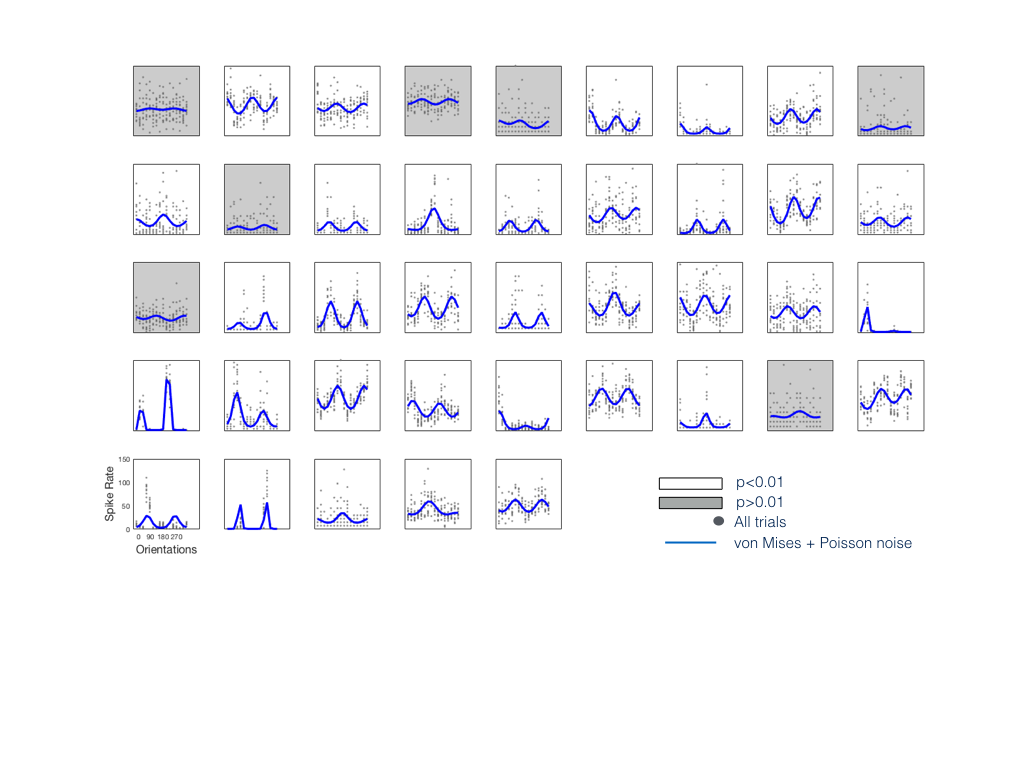
\includegraphics[width=1\linewidth]{BIG1.png}
\caption{ All cells with original spike count for each trial (grey dot) and tuning curves (blue line). Significantly orientation-selective neurons in white frames, non-significant cells in grey frames.}
\end{figure}

\bibliography{Report}


\end{document}